\chapter{Resultados Parciais}

Este capítulo é destinado aos resultados obtidos através dos experimentos descritos anteriormente Observe na figura \ref{fig:graph_result} e na tabela \ref{tab:results_table} abaixo uma comparação entre os modelos de classificação avaliados utilizando as cinco métricas adotadas no projeto.

\begin{figure}[!htb]
    \center{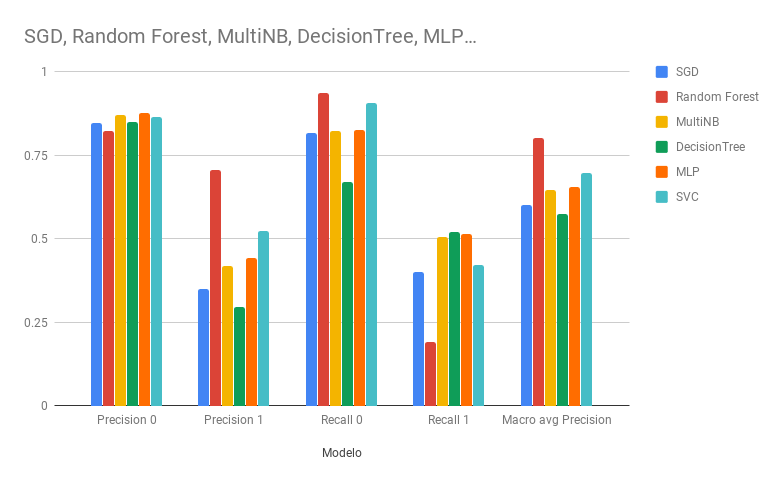
\includegraphics[scale=0.6]
    {figuras/graph_result.png}}
    \caption{\label{fig:graph_result} Gráfico com o resultado dos métodos.}
\end{figure}

\begin{table}[!htb]
\begin{tabular}{|l|l|l|l|l|l|}
\hline
Modelo & Precision 0 & Precision 1 & Recall 0 & Recall 1 & \begin{tabular}[c]{@{}l@{}}Macro avg\\ Precision\end{tabular} \\ \hline
\cellcolor[HTML]{3166FF}SGD & 0.848 & 0.35 & 0.816 & 0.402 & 0.6 \\ \hline
\cellcolor[HTML]{CB0000}Random Forest & 0.824 & 0.706 & 0.938 & 0.19 & 0.802 \\ \hline
\cellcolor[HTML]{FCFF2F}MultiNB & 0.872 & 0.418 & 0.822 & 0.506 & 0.646 \\ \hline
\cellcolor[HTML]{32CB00}Decision Tree & 0.85 & 0.296 & 0.67 & 0.52 & 0.574 \\ \hline
\cellcolor[HTML]{F8A102}MLP & 0.876 & 0.442 & 0.826 & 0.514 & 0.656 \\ \hline
\cellcolor[HTML]{00D2CB}SVC & 0.866 & 0.522 & 0.906 & 0.422 & 0.698 \\ \hline
\end{tabular}
\caption{Tabela com o resultado dos métodos}
\label{tab:results_table}
\end{table}

Através desses dados, é possível identificar que o modelo do Random Forest se destacou dos demais por sua precisão ao identificar a classe 1. Isso significa que, ao classificar um comentário como discurso de ódio, este modelo é, relativamente, confiável. Porém, o Recall da classe 1 esteve abaixo da média, mostrando uma tendência ao falso negativo para a mesma classe, ou seja, altas chances de se deixar passar um discurso de ódio.

Enquanto o Random Forest se destaca pela disparidade em uma das métricas, o modelo Multi-Layer Perceptron (MLP) se apresenta com bons valores para o recall da classe 1, sem comprometer as outras métricas. Ao compará-lo com os outros modelos, ele apresenta entre os melhores em todas as cinco métricas exibidas acima.


